\chapter{Artifact Detection and Localization}

The artifact detection and localization pipeline is responsible for converting the sensor data from the various payloads (Mk. 0, Mk. 1, drone), into a list of artifacts to send to the base station and ultimately report to DARPA. The pipeline was developed to meet a set of requirements, which were derived from the competition rules and our team's concept of operations:

\begin{enumerate}
	\item Reported coordinate of artifact must be within 5m (Euclidean distance) of DARPA-surveyed coordinate
	\item Pipeline must run on-board, either on the Xavier (Mk. 0, Mk. 1), or on part of the NUC (drone)
	\item Artifacts must be transmitted to base station over a lossy wireless link
	\item Pipeline should be capable of detecting all 5 types of artifacts (as shown in Figure \ref{tunnel artifacts})
	\item All artifacts which the robots pass by should be detected
	\item Pipeline should be identical or nearly identical on all payloads
	\item Artifacts should be detected and reported to human supervisor in real-time
\end{enumerate}

Additionally, the following assumptions were made to constrain the scope of the pipeline and guide parameter tuning wherever necessary:

% TODO(vasua): Turn this (and above) into a table
\begin{enumerate}
	\item State estimation system on all payloads would be LOAM
	\item Artifact detection and localization pipeline could not direct robots' exploration
	\item Artifacts are reported in robots' own frames and transformed to a single world frame at base station
	\item Robots will move at approximately 2 m/s
	\item A human supervisor would be available to verify artifact reports, and thus false positives are acceptable
\end{enumerate}

An overview of the complete pipeline is given in Figure \ref{software_overview}. This pipeline runs identically on all 3 payloads with only minor configuration changes (e.g. sensor serial numbers), and sensor omissions where necessary (e.g. drone payload does not contain a thermal camera). All robots report artifacts to the GUI independently, and no information is shared between pipelines running on individual payloads.

\begin{figure}	
	\centering
	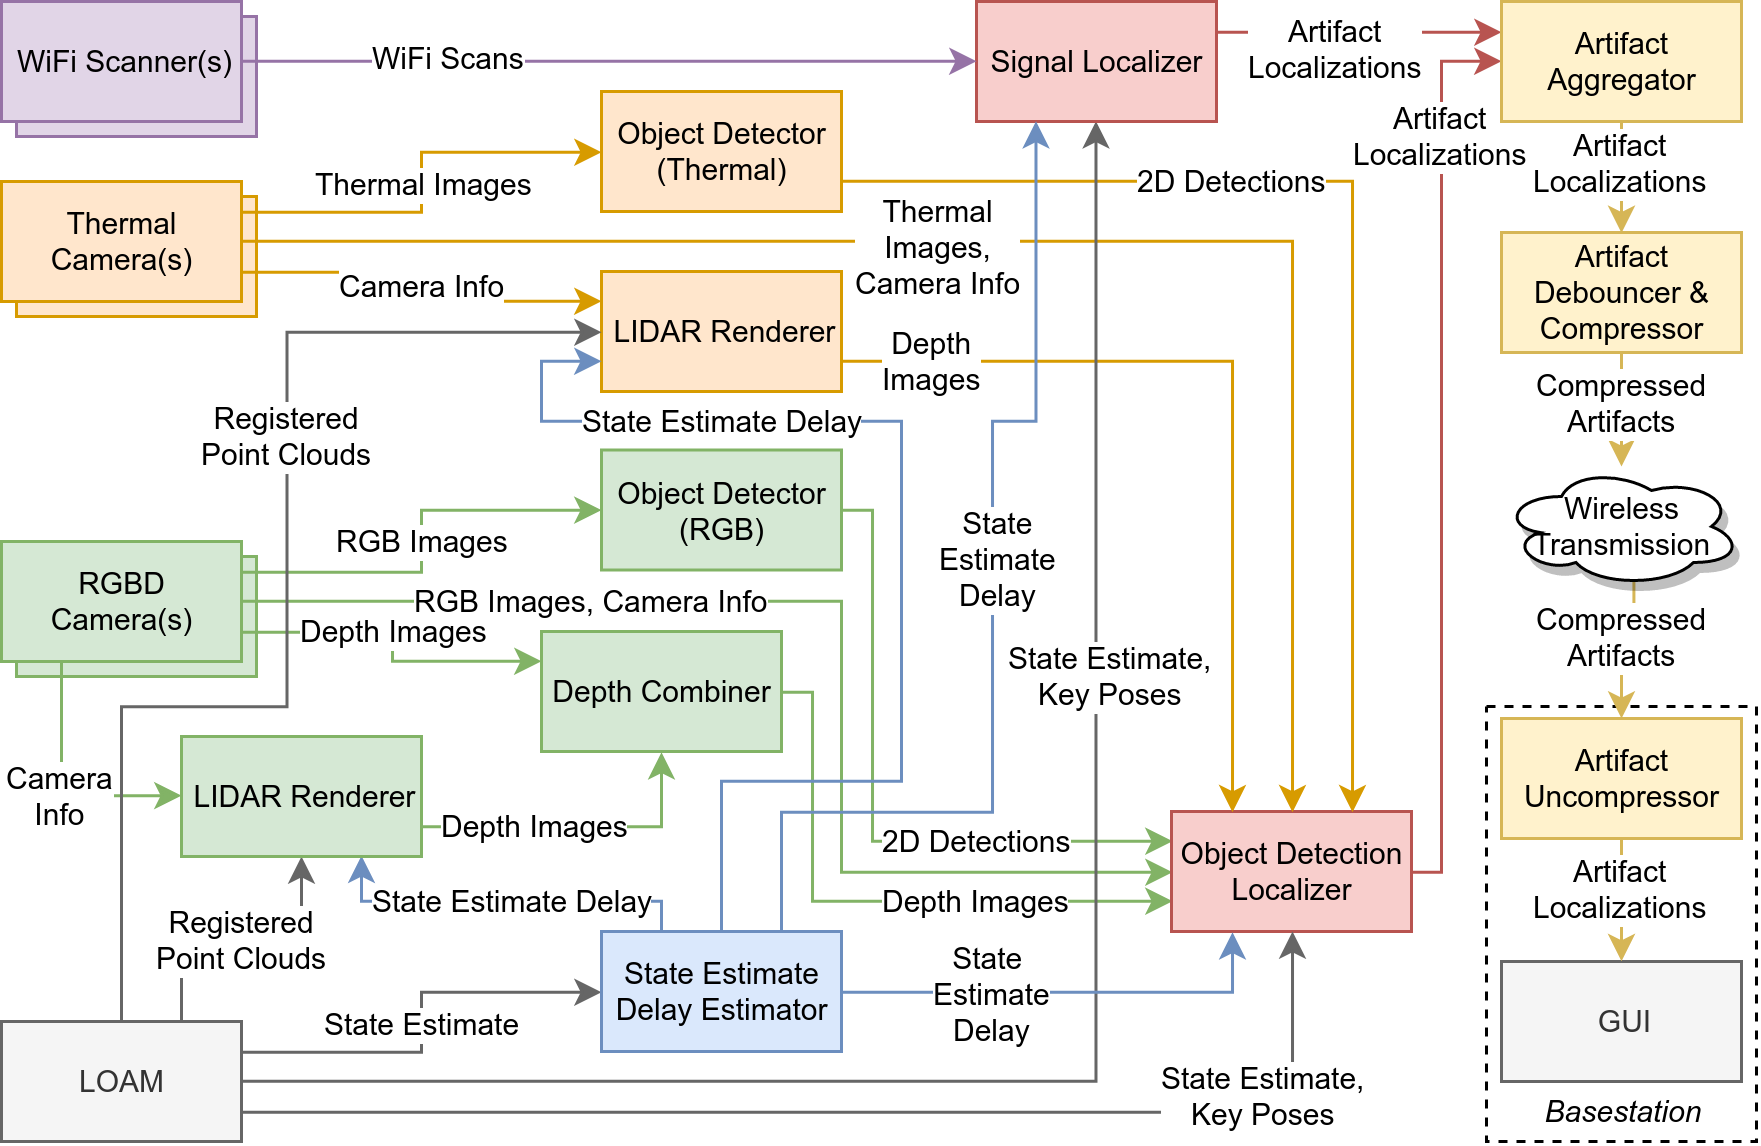
\includegraphics[width=\textwidth]{software_overview.png}
	\caption{Artifact detection and localization software diagram}
	\label{software_overview}
\end{figure}

% TODO(vasua): A better figure for what is inside an artifact localization?
The pipeline consists of 2 major modules - the Signal Localizer and the Object Detection Localizer. Each module takes in various sensor data and produces Artifact Localizations, which are 3D coordinates in the robot's map frame that are believed to correspond to a desired artifact. These Artifact Localizations may contain additional evidence to be displayed to the human supervisor, such as images or point clouds of the artifact and surrounding environment. Artifact Localizations from both modules are combined inside the Artifact Aggregator and then transmitted to the base station to be displayed on the GUI. The human supervisor inspects artifacts displayed on the GUI and reports valid ones to DARPA.

\section{LOAM Overview}

One of the assumptions made during the initial design phases of the software pipeline was that LOAM would be the state estimation system used on all of our payloads. This simplified the development of the artifact detection and localization pipeline as we only needed to develop and test against a single state estimation system. The relevant interface details of LOAM (in the form of ROS frames and topics) are given below:

\begin{description}
	\item[/sensor] This is the robot's local frame, and is coincident with the Velodyne LIDAR's frame.
	\item[/sensor\_init] The fixed frame used as the base for LOAM's odometry.
	\item[/map] The world frame, which is initially coincident with sensor\_init but can change after loop closures.
	\item[/key\_pose\_to\_map] LOAM creates a series of key poses as the robot traverses the environment. These key poses are generated approximately every 2 meters of the robot's path. Each key pose is given a unique ID, starting from 0. The key pose is published relative to the /map frame.
	\item[/key\_pose\_path] When LOAM detects a loop closure, it corrects the key poses and publishes a new list of key pose IDs and poses.
	\item[/velodyne\_cloud\_registered] The laser scan from the Velodyne LIDAR is aligned to previous scans and published on this topic at 5 Hz. Registered scans are published on this topic even when the robot is stationary. The scans are registered in the /sensor\_init frame and accumulate drift over time, but are locally smooth.
	\item[/integrated\_to\_map] The 6DOF pose of the /sensor frame is published on this topic at 200 Hz. The pose is corrected by loop closures and thus does not accumulate significant drift, but may be discontinuous locally.
\end{description}

\section{Object Detector (RGB)}

\subsection{Network Benchmarks}
\subsection{Data Collection and Labeling}
\subsection{Training}
\subsection{Evaluation}

\section{Object Detector (Thermal)}
TODO

\section{LIDAR Renderer}

The LIDAR renderer uses camera information (intrinsics and extrinsics) to render depth images. The depth information comes from the registered point clouds from LOAM. For RGB images, the LIDAR renderer provides an alternative source for depth information as depth images are already produced by the RealSense cameras. However, the LIDAR renderer serves as the only source of depth information for the thermal cameras, as they do not otherwise have associated depth information.

\subsection{Method}

Two implementations of the LIDAR renderer were created - a reference implementation which ran on CPU, and an optimized one which ran on a GPU using CUDA. The optimized implementation is used on both Mk. 0 and Mk. 1 and runs on the Xavier, where it renders depth images for either 5 or 6 image streams (4x RGB and 1 or 2x thermal). The reference implementation was used to validate the GPU implementation for correctness. The reference implementation also runs on the NUC on the drone payload as it does not have a GPU that supports CUDA. The slower performance of the reference implementation is acceptable as renders only need to be produced for a single RGB stream. Both implementations share the same overall algorithm, comprising two separate methods:

\begin{description}
	\item[Cloud aggregation] The renderer aggregates the registered point clouds from LOAM. A rolling buffer of these clouds is maintained, whose size is proportional to the time it takes to render an image. 10 clouds are stored in the reference implementation, and 30 clouds are stored in the GPU implementation. The clouds are already transformed into a common frame and form a locally smooth point cloud. Global drift is present, but can be ignored since the rendered depth images only see a small local portion of the map.
	\item[Rendering] For each rendered image, the renderer computes the position of the camera in the same frame as the aggregated point clouds. The renderer then uses the camera intrinsics to construct a pinhole camera model and projects each point through it to obtain a location in image coordinates. This coordinate, as well as pixels around this coordinate (based on a configurable inflation parameter) are updated based on the distance to the point, keeping the closer point. The projected coordinates are inflated (as shown in Figure \ref{lidar_inflate}) to provide a denser output image to ensure that depth values are not lost in any potential future downsampling.
\end{description}

\begin{figure}
	\centering
	\begin{subfigure}{0.3\textwidth}
		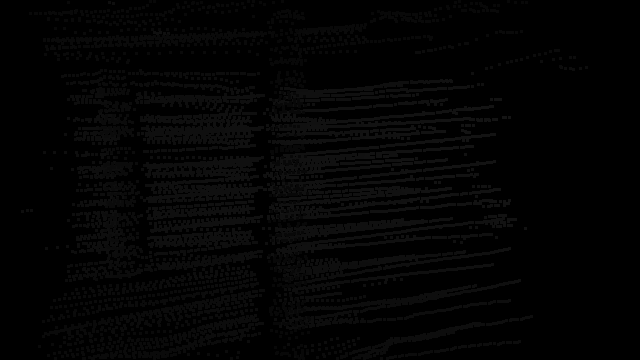
\includegraphics[width=\textwidth]{inflate_1.png}
		\caption{1 pixel inflation}
		\label{inflate_1}
	\end{subfigure}		
	\hfill
	\begin{subfigure}{0.3\textwidth}
		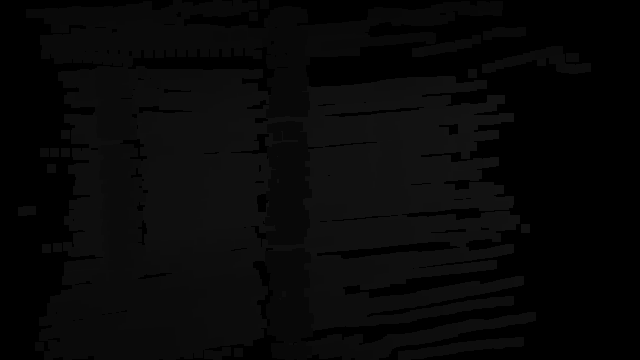
\includegraphics[width=\textwidth]{inflate_4.png}
		\caption{4 pixel inflation}
		\label{inflate_4}		
	\end{subfigure}
	\hfill
	\begin{subfigure}{0.3\textwidth}
		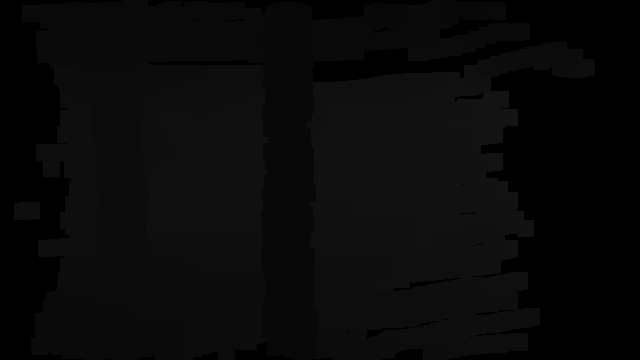
\includegraphics[width=\textwidth]{inflate_8.png}
		\caption{8 pixel inflation}
		\label{inflate_8}
	\end{subfigure}
	\caption[LIDAR renderer inflation values comparison]{Rendered images of the same scene with different inflation values. An inflation value of 4 was used for all payloads.}
	\label{lidar_inflate}
\end{figure}

\subsection{Results}

A selection of outputs from the LIDAR renderer is given in Figure \ref{lidar_renderer_images}, along with the depth image output from the RealSense camera and the associated RGB image for reference. In the first row, with Mk. 1's camera looking down a long tunnel, the rendered image is significantly sharper and more consistent than that of the RealSense. In the second row, with the left camera looking at a nearby wall, both depth images are similar. In the final row, with a scene from Mk. 1's back camera (which is tilted upwards), the RealSense depth image has significantly fewer holes than the LIDAR's due to the LIDAR's narrow vertical field of view. 

These results show that the output from the LIDAR renderer is either on par with, or better than that from the RealSense cameras, assuming the camera's full field of view is captured by the LIDAR. By fusing both depth images in the Depth Combiner, we can obtain better depth images than either source provides individually.

\begin{figure}
	\centering
	\begin{subfigure}{0.3\textwidth}
		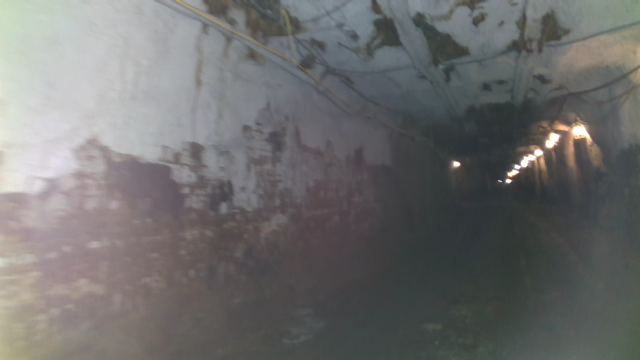
\includegraphics[width=\textwidth]{rs_front_example_2019-10-16-00-51-04_color.png}
		\caption{Mk. 1 Front Color}
		\label{lidar_front_color}
	\end{subfigure}		
	\hfill
	\begin{subfigure}{0.3\textwidth}
		
\includegraphics[width=\textwidth]{rs_front_example_2019-10-16-00-51-04_ref.png}
		\caption{Mk. 1 Front Depth}
		\label{lidar_front_ref}		
	\end{subfigure}
	\hfill
	\begin{subfigure}{0.3\textwidth}
		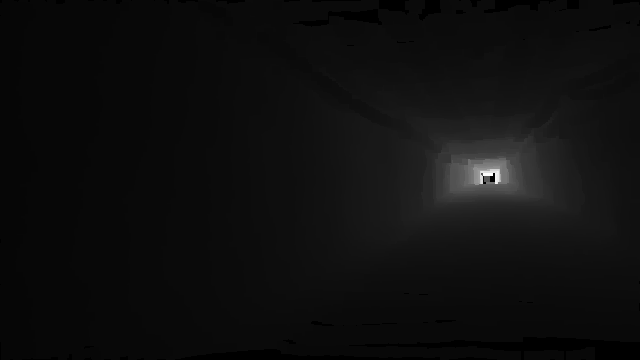
\includegraphics[width=\textwidth]{rs_front_example_2019-10-16-00-51-04_render.png}
		\caption{Mk. 1 Front Rendered}
		\label{lidar_front_render}
	\end{subfigure}
	\\
	\begin{subfigure}{0.3\textwidth}
		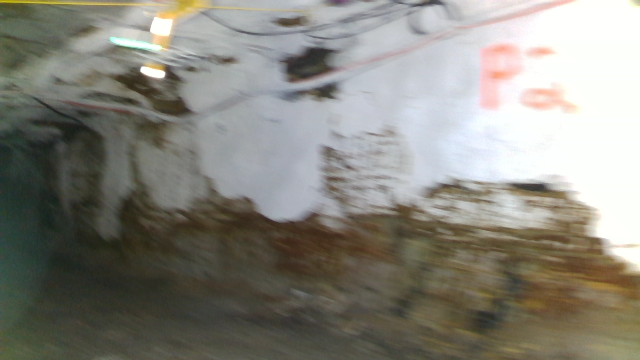
\includegraphics[width=\textwidth]{rs_left_example_2019-10-16-00-51-02_color.png}
		\caption{Mk. 1 Left Color}
		\label{lidar_left_color}
	\end{subfigure}		
	\hfill
	\begin{subfigure}{0.3\textwidth}
		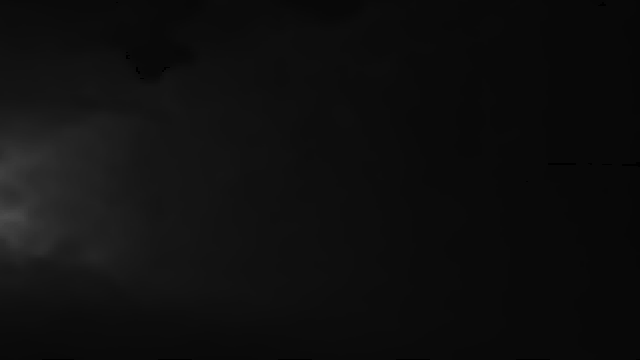
\includegraphics[width=\textwidth]{rs_left_example_2019-10-16-00-51-02_ref.png}
		\caption{Mk. 1 Left Depth}
		\label{lidar_left_ref}		
	\end{subfigure}
	\hfill
	\begin{subfigure}{0.3\textwidth}
		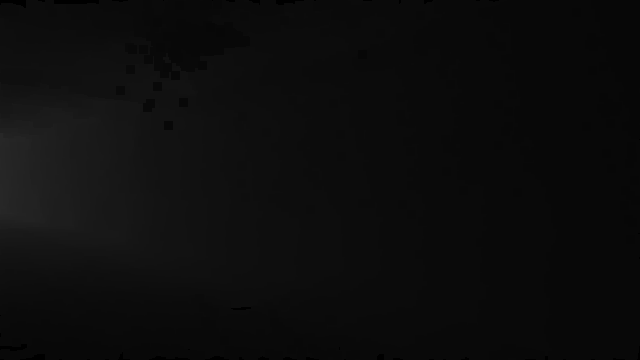
\includegraphics[width=\textwidth]{rs_left_example_2019-10-16-00-51-02_render.png}
		\caption{Mk. 1 Left Rendered}
		\label{lidar_left_render}
	\end{subfigure}
	\\
	\begin{subfigure}{0.3\textwidth}
		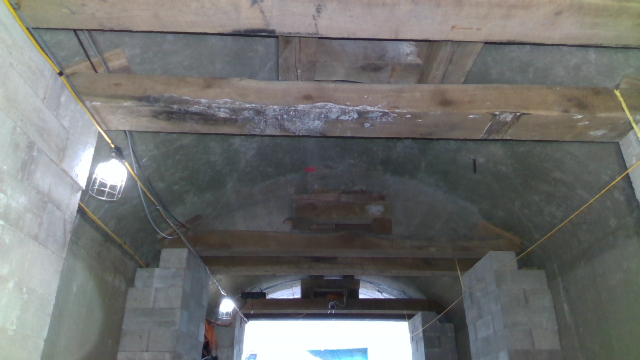
\includegraphics[width=\textwidth]{rs_back_example_2019-10-16-00-33-41_color.png}
		\caption{Mk. 1 Back Color}
		\label{lidar_back_color}
	\end{subfigure}		
	\hfill
	\begin{subfigure}{0.3\textwidth}
		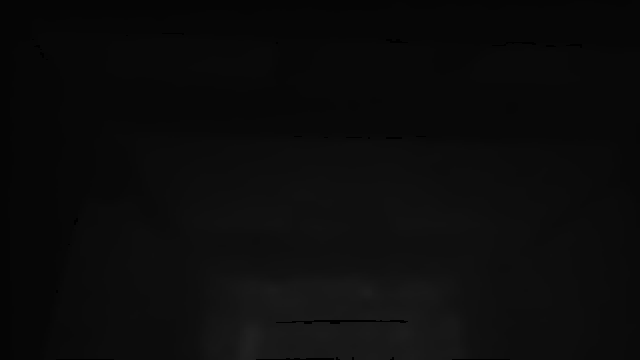
\includegraphics[width=\textwidth]{rs_back_example_2019-10-16-00-33-41_ref.png}
		\caption{Mk. 1 Back Depth}
		\label{lidar_back_ref}		
	\end{subfigure}
	\hfill
	\begin{subfigure}{0.3\textwidth}
		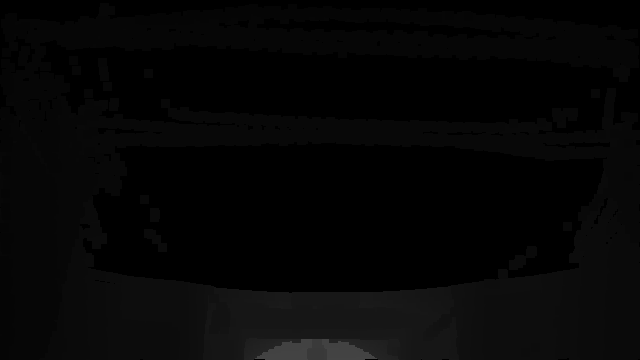
\includegraphics[width=\textwidth]{rs_back_example_2019-10-16-00-33-41_render.png}
		\caption{Mk. 1 Back Rendered}
		\label{lidar_back_render}
	\end{subfigure}		
	\caption[LIDAR renderer depth image comparison]{Comparison of depth images generated by the LIDAR renderer to depth images from the RealSense cameras. Color images, captured simultaneously by the RealSense cameras, are provided for reference.}
	\label{lidar_renderer_images}
\end{figure}

\section{Depth Combiner}

The depth combiner fuses depth images from the RealSense depth camera and LIDAR renderer into a single depth image to be used in the object detection localizer. The two image streams are aligned, and can thus be fused per-pixel. The following equation was used (shown as C++ code):

\begin{lstlisting}[language=c++]
fused = (realsense > threshold || realsense == 0) ? lidar : realsense;
\end{lstlisting}

This fusion keeps LIDAR data whenever the reported RealSense data is either not present (\lstinline[language=c++]{realsense == 0}) or exceeds some threshold (\lstinline[language=c++]{realsense > threshold}). The threshold was empirically selected to be 2.5m, which is the approximate distance after which we observed significant variance in reported depth values between frames. This fusion allows us to use the high density RealSense depth information whenever it is available and sufficiently accurate (under the 2.5m threshold), and utilize the sparser LIDAR information otherwise. An example output is given in Figure \ref{combined_depth}.

\begin{figure}
	\centering
	\begin{subfigure}{0.3\textwidth}
		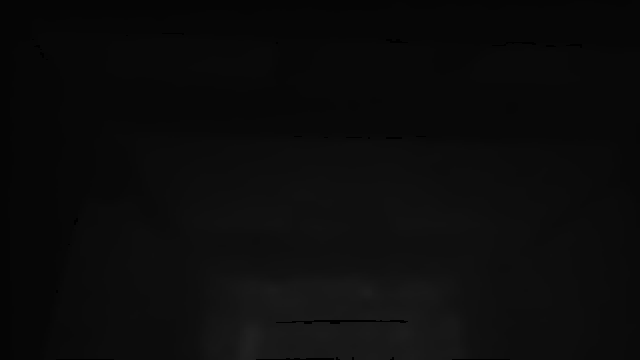
\includegraphics[width=\textwidth]{rs_back_example_2019-10-16-00-33-41_ref.png}
		\caption{Mk. 1 Back Depth}
		\label{combined_depth_realsense}		
	\end{subfigure}
	\hfill
	\begin{subfigure}{0.3\textwidth}
		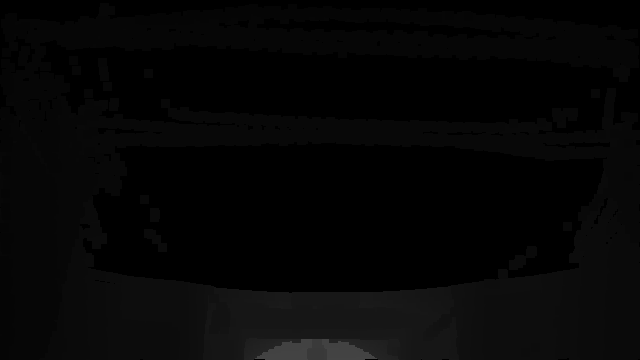
\includegraphics[width=\textwidth]{rs_back_example_2019-10-16-00-33-41_render.png}
		\caption{Mk. 1 Back Rendered}
		\label{combined_depth_lidar}
	\end{subfigure}	
	\hfill
	\begin{subfigure}{0.3\textwidth}
		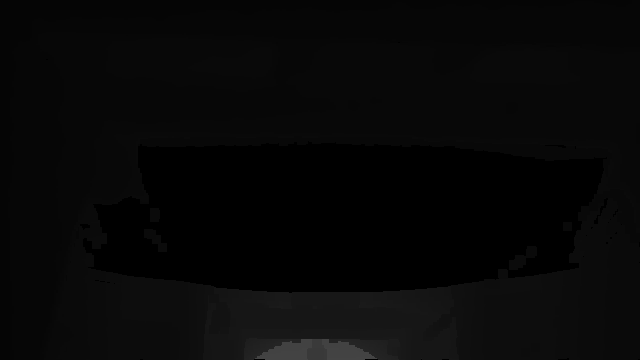
\includegraphics[width=\textwidth]{combined_depth.png}
		\caption{Mk. 1 Back Combined}
		\label{combined_depth_output}
	\end{subfigure}		
	\caption[Depth combiner sample output]{Example of the output from the depth combiner, using the same scene as in \ref{lidar_back_color}.}
	\label{combined_depth}
\end{figure}


\section{Object Detection Localizer}

The object detection localizer aggregates multiple 2d object detections in the RGB and thermal images and produces candidate Artifact Localizations. The localizer is able to combine detections of the same object from different camera streams together into a single Artifact Localization. Once sufficient evidence has been obtained for an Artifact Localization, the localizer will publish it to the Artifact Aggregator. Artifact Localizations are updated at 1 Hz using key pose information from LOAM to ensure global correctness for the duration of the robots' exploration. Significant changes in artifact positions are published to the Artifact Aggregator to be sent to the human operator to verify.

For any potential artifact, evidence is only accumulated in the form of positive detections from the object detectors. Negative detections do not reduce the likelihood that an artifact is present at a given location. This biases the object detection localizer to return a large number of false positives, as most spurious detections from the object detectors will get reported as Artifact Localizations to the base station. This approach was consistent with our requirements and assumptions - as the human supervisor was able to validate artifact reports, even a large number of false positives was acceptable if it meant that no artifacts were missed.

\subsection{Method}

The object detection localizer consists of 3 main operations, separated into two threads. The first thread, running the key pose maintenance and detection backprojection tasks, is responsible for creating and maintaining a data structure which stores a 3d point cloud associated with each 2d detection with respect to a key pose. The second thread, running the clustering task, is responsible for extracting new Artifact Localizations from the data structure, updating existing ones, and publishing changes. The clustering task's execution time scales with the size of the data structure and thus runs in a separate thread, ensuring that all callbacks in the primary thread are serviced in time.

\begin{description}
	\item[Key Pose Maintenance] The key pose maintenance task is responsible for populating and updating a data structure with key pose information from LOAM. When key poses are initially received, they contain a timestamp and an ID in addition to the pose information. Both pieces of metadata are stored alongside the key pose. The ID is used to update the corresponding key poses when a list of updated key poses is received from LOAM after a loop closure. The timestamp is made available to other tasks to be able to associate other sensor measurements to a key pose.
	
	\item[Detection Backprojection] The detection backprojection task runs as a callback upon receiving a set of 2d object detections, a color image, an associated depth image, and camera intrinsics information. For each detection, the depth information and camera intrinsics are used to project all pixels which fall inside the bounding box through a pinhole model into a 3d point cloud in the camera frame. The point cloud is colored by the RGB image, and each point in the cloud is assigned an ID corresponding to the classification of the detection. The timestamp of the image frame is then used to look up the immediately preceding key pose in the structure built by the key pose maintenance task. The point cloud is then transformed to be in the key pose's frame, and is added to a list of point clouds associated with that particular key pose. The color image has the bounding box drawn on it, and is stored alongside the point cloud. The centroid of the point cloud is also computed and stored, to enable more efficient clustering. This backprojection process is identical for both RGB and thermal images.
	
	It is important that the backprojected point clouds are stored relative to a particular key pose rather than relative to the overall /map frame. The transform necessary to convert the point cloud into the key pose frame is obtained in two steps. First, the static transform from the camera to the LOAM sensor frame is combined with the \textbf{/integrated\_to\_map} frame at the image timestamp, yielding a transform from the camera frame to the /map frame. Then, the pose of the corresponding key pose (which is already in the /map frame) is used to create a transform from the camera frame to the key pose frame. Storing the backprojected point clouds relative to a key pose rather than directly in the /map frame allows the clouds to be more accurately transformed into the /map frame as the key poses are updated. By using the \textbf{/integrated\_to\_map} topic, we ensure that the error the eventual transformation into the /map frame is due to small IMU integration error between key poses, rather than a large global drift.
	
	Some additional filtering is also performed during this step to improve the quality of data being stored. The robot's pose estimate must move by a small amount (empirically selected to be 7.5cm) between frames, or clouds are not generated at all. This threshold ensures that redundant information does not get stored if the robot is sitting still or moving very slowly. Additionally, depending on the source of depth information being used, different downsampling and depth cutoff parameters are used in the backprojection. Downsampling reduces the density of the backprojected point cloud by skipping certain pixels when backprojecting. Every 4th row and column is kept when utilizing RealSense depth information, while every 2nd row and column is kept when using the comparatively sparse LIDAR rendered depth information. The depth cutoff is used to discard any points which have depth values beyond a certain point, and is used to compensate for low accuracy in the depth values. A depth cutoff of 10m was selected, intended to only act as a cutoff for the LIDAR depth values as a lower cutoff was used in the Depth Combiner when fusing the RealSense depth data.
	
	\item[Clustering] The clustering task continually (at 1 Hz) creates Artifact Localizations from the data structure populated by the backprojection task, and publishes deltas for downstream nodes to use. First, the centroid of each backprojected point cloud is transformed into the /map frame using the updated pose of the corresponding key pose. This centroid cloud is then clustered using Euclidean clustering from PCL, with a cluster tolerance of 0.5m and a minimum cluster size of 3. These parameters group objects which have been detected a sufficient number of times (3) and are close enough (0.5m) together. The clustering is purely geometric, and does not account for the classification of the centroid. This choice enables the clustering process to be more robust to misclassification from the network, but in exchange sacrifices the ability to distinguish multiple objects of different types near each other.
	
	The centroid of each cluster can be treated as an approximation for the centroid of each artifact that the robot has seen. However, the computed centroid of centroids is imprecise, and can be refined by integrating the complete point clouds for each detection. First, the clouds are transformed into the /map frame and aggregated into a single cloud for the cluster. The centroid of this cloud is then found, and used as the refined position of an Artifact Localization. This centroid differs from the one computed using the centroid of each point cloud as it will weight the centroids based on the number of points in the cloud, rather than weighting all centroids equally. While finding the centroid of the cluster point cloud, a majority vote is performed over the classifications to determine a label for the Artifact Localization. Finally, the color images (with bounding boxes) for each detection in the cluster are added to the Artifact Localization as evidence.
	
	Once the complete list of Artifact Localizations has been created from the available data, it is compared against existing valid Artifact Localizations generated by previous iterations. New Artifact Localizations are matched pairwise against previous ones, again only considering Euclidean distance, using a threshold of 0.25m. Previous Artifact Localizations which are matched to new ones have their parameters updated with the ones of their match. Previous ones which were not matched are now considered invalid, and are marked as such, but are not forgotten. New Artifact Localizations which did not match any previous ones are given a new ID and stored as valid Artifact Localizations. All changes to Artifact Localizations (updates, invalidations, and new ones) are published, along with the IDs of each Artifact Localization. This process of publishing deltas in the list of Artifact Localizations is used to increase memory efficiency and reduce transmission bandwidth.
	
	When publishing Artifact Localizations, only a small number of images are kept. Typically, an Artifact Localization will amass 50 or more detections from different cameras as the robot drives by an artifact. These images are highly redundant, and it is thus inefficient to transmit them all. Instead, only 4 selected images are published. The images are sorted by their capture timestamp and then evenly distributed into 4 chunks. The first image from each chunk is kept, ideally resulting in images which show multiple perspectives of an artifact as the robot travels by. An example of 4 automatically selected images for an artifact is shown in Figure \ref{automatically_selected_images}.
\end{description}

\begin{figure}
	\centering
%	\begin{subfigure}{0.4\textwidth}
%		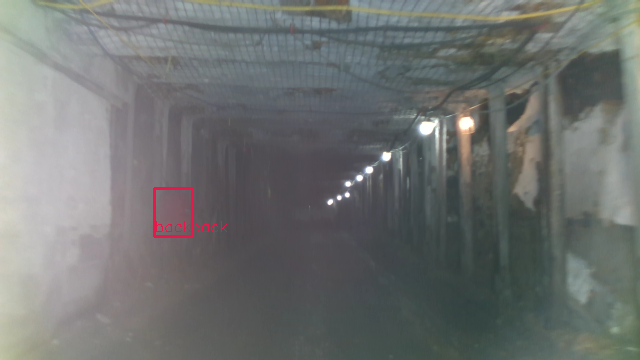
\includegraphics[width=\textwidth]{artifact_0003_image_00.png}
%%		\caption{Backpack Image 1}
%		\label{backpack_image_1}
%	\end{subfigure}		
%	\hfill
%	\begin{subfigure}{0.4\textwidth}
%		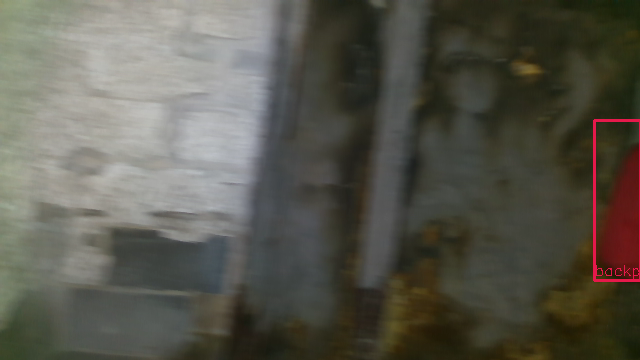
\includegraphics[width=\textwidth]{artifact_0003_image_01.png}
%%		\caption{Backpack Image 2}
%		\label{backpack_image_2}
%	\end{subfigure}
%	\\
%	\begin{subfigure}{0.4\textwidth}
%		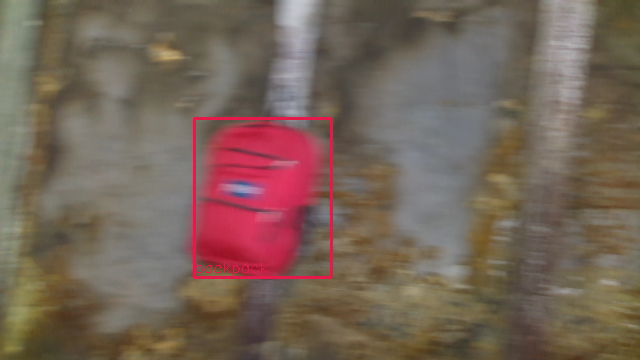
\includegraphics[width=\textwidth]{artifact_0003_image_02.png}
%%		\caption{Backpack Image 3}
%		\label{backpack_image_3}
%	\end{subfigure}
%	\hfill
%	\begin{subfigure}{0.4\textwidth}
%		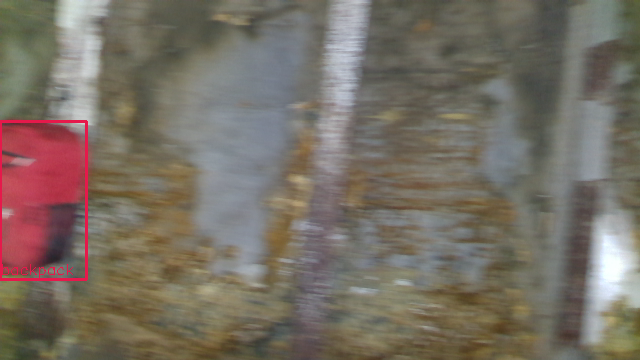
\includegraphics[width=\textwidth]{artifact_0003_image_03.png}
%%		\caption{Backpack Image 4}
%		\label{backpack_image_4}
%	\end{subfigure}
%	\\
	\begin{subfigure}{0.45\textwidth}
		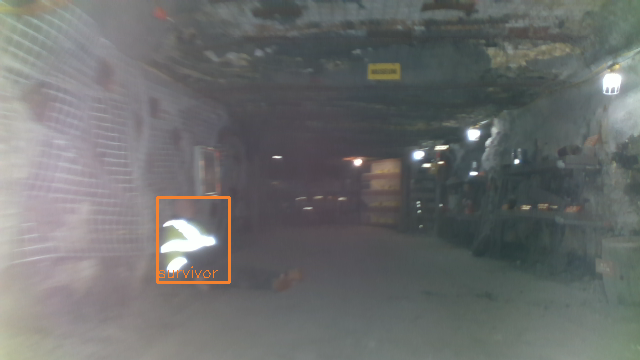
\includegraphics[width=\textwidth]{artifact_0019_image_00.png}
		\caption{Survivor Image 1}
		\label{survivor_image_1}
	\end{subfigure}		
	\hfill
	\begin{subfigure}{0.45\textwidth}
		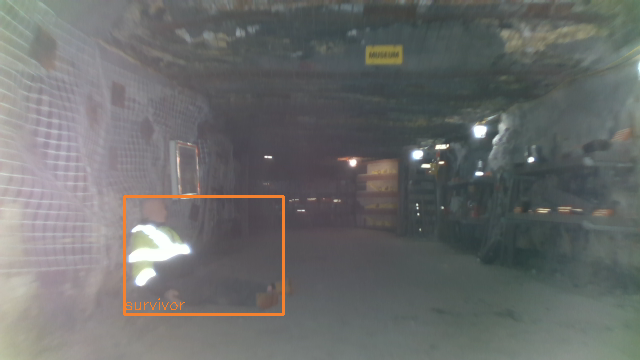
\includegraphics[width=\textwidth]{artifact_0019_image_01.png}
		\caption{Survivor Image 2}
		\label{survivor_image_2}
	\end{subfigure}
	\\
	\begin{subfigure}{0.45\textwidth}
		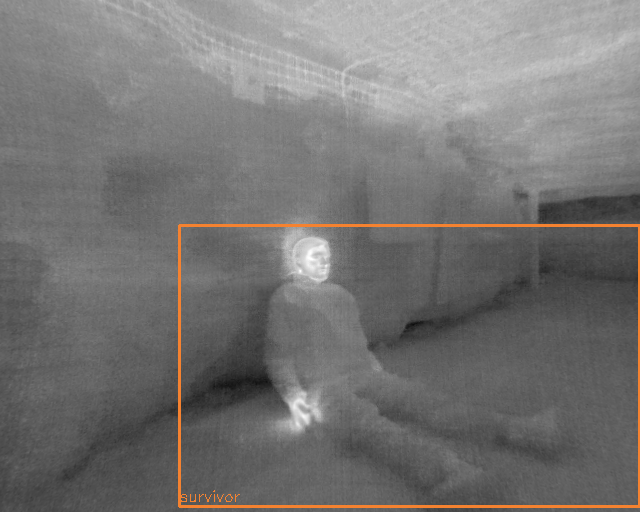
\includegraphics[width=\textwidth]{artifact_0019_image_02.png}
		\caption{Survivor Image 3 (thermal)}
		\label{survivor_image_3}
	\end{subfigure}
	\hfill
	\begin{subfigure}{0.45\textwidth}
		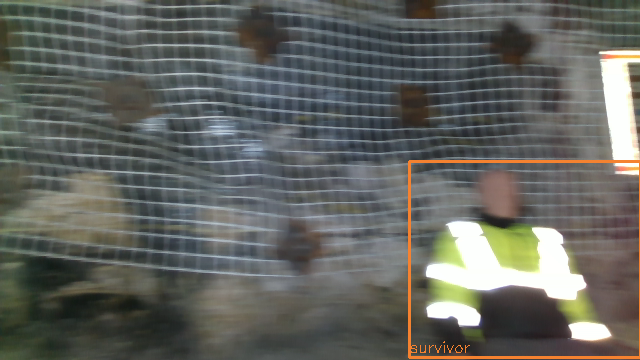
\includegraphics[width=\textwidth]{artifact_0019_image_03.png}
		\caption{Survivor Image 4}
		\label{survivor_image_4}
	\end{subfigure}		
	\caption[Automatically selected images from Artifact Localizations]{Each published Artifact Localization contains only a few images automatically selected from the many detections which combine together to form a single Artifact Localization. These images can be selected across different cameras and different types of cameras, as shown above.}
	\label{automatically_selected_images}
\end{figure}

\subsection{Results}

\section{WiFi Scanner}

TODO

\section{Signal Localizer}

TODO

\section{State Estimate Delay Estimator}

TODO

\section{Artifact Aggregator}

TODO

\section{Artifact Debouncer \& Compressor}

TODO

\section{Artifact Uncompressor}

TODO

\section{GUI}